\documentclass[aspectratio=169]{beamer}

% Shared Beamer settings for Applied Machine Learning lectures (UPES).
% Keep this file free of \documentclass to allow reuse via \input.

% Allow lecture sources to use shared theme/assets without copying them into each lecture folder.
% NOTE: These paths are relative to `Unit-xx/Lecture-yy/latex/` (and `Lab/Experiment-xx/latex/`).
\makeatletter
\def\input@path{{../../../_shared/}{../../../_shared/UPES-Beamer-Theme/}}
\makeatother

\usetheme{UPES}
\setbeamertemplate{navigation symbols}{}

\usepackage{amsmath}
\usepackage{amssymb}
\usepackage{booktabs}
\usepackage{graphicx}
\usepackage{hyperref}
\usepackage{xcolor}
\usepackage{listings}

% Code listings (Python-oriented for this subject).
\lstset{
  language=Python,
  basicstyle=\ttfamily\small,
  keywordstyle=\color{blue},
  commentstyle=\color{gray},
  stringstyle=\color{teal},
  showstringspaces=false,
  columns=fullflexible,
  breaklines=true
}

\usepackage{tikz}
\usetikzlibrary{arrows.meta,positioning,shapes.geometric,calc,fit,backgrounds}

% Per-slide source line (references shown on the slide itself).
\newcommand{\slidesources}[1]{%
  \vfill
  {\tiny\color{gray}\raggedright\sloppy\parbox{\linewidth}{Sources: #1}\par}%
}

% Unit-wise source strings for this subject (used by slides/notes).
% Path is relative to the lecture `latex/` folder (the compilation CWD).
% Source strings for Applied Machine Learning (CSAI2017P) — used by slides + notes.
% Prescribed texts and reference books are taken from the course syllabus.
% Support texts are the author-hosted open-access editions:
%   statlearning.com            (ISL with Python)
%   probml.github.io/pml-book   (Murphy, Probabilistic Machine Learning)
%   d2l.ai                      (Dive into Deep Learning)
%   mml-book.github.io          (Mathematics for Machine Learning)

\newcommand{\AMLRepoURL}{https://github.com/tali7c/Applied-Machine-Learning}

% --- prescribed -------------------------------------------------------------
\newcommand{\AMLPrescribed}{%
M\"uller and Guido, \textit{Introduction to Machine Learning with Python}, O'Reilly, 2016.;%
Bishop, \textit{Pattern Recognition and Machine Learning}, Springer, 2006.;%
Murphy, \textit{Machine Learning: A Probabilistic Perspective}, MIT Press, 2012.;%
Han, Kamber and Pei, \textit{Data Mining: Concepts and Techniques} (3e), Morgan Kaufmann, 2012.%
}

% --- unit-wise ---------------------------------------------------------------
\newcommand{\AMLUnitISources}{%
M\"uller and Guido, \textit{Introduction to Machine Learning with Python}, Ch. 1.;%
Bishop, \textit{Pattern Recognition and Machine Learning}, Ch. 1.;%
Murphy, \textit{Probabilistic Machine Learning: An Introduction}, MIT Press, 2022, Ch. 1.;%
Mitchell, \textit{Machine Learning}, McGraw Hill, 1997, Ch. 1.;%
Scikit-learn documentation, accessed 2026-08-04.%
}

\newcommand{\AMLUnitIISources}{%
Bishop, \textit{Pattern Recognition and Machine Learning}, \S1.5, \S4.3, \S7.1.;%
Zhang, Lipton, Li and Smola, \textit{Dive into Deep Learning}, \S3.4.;%
Shalev-Shwartz and Ben-David, \textit{Understanding Machine Learning}, Ch. 15.;%
Murphy, \textit{Probabilistic Machine Learning: An Introduction}, Ch. 5.%
}

\newcommand{\AMLUnitIIISources}{%
Zhang, Lipton, Li and Smola, \textit{Dive into Deep Learning}, Ch. 12 (Optimization Algorithms).;%
Deisenroth, Faisal and Ong, \textit{Mathematics for Machine Learning}, Ch. 7.;%
Kingma and Ba, ``Adam: A Method for Stochastic Optimization,'' ICLR 2015.;%
Ruder, ``An overview of gradient descent optimization algorithms,'' arXiv:1609.04747, 2016.%
}

\newcommand{\AMLUnitIVSources}{%
Han, Kamber and Pei, \textit{Data Mining: Concepts and Techniques} (3e), Ch. 3.;%
M\"uller and Guido, \textit{Introduction to Machine Learning with Python}, Ch. 3--4.;%
James, Witten, Hastie, Tibshirani and Taylor, \textit{An Introduction to Statistical Learning with Python}, Ch. 5--6, 12.;%
Scikit-learn documentation (preprocessing, model selection), accessed 2026-08-04.%
}

\newcommand{\AMLUnitVSources}{%
James et al., \textit{An Introduction to Statistical Learning with Python}, Ch. 3--6.;%
Bishop, \textit{Pattern Recognition and Machine Learning}, Ch. 3.;%
Deisenroth, Faisal and Ong, \textit{Mathematics for Machine Learning}, Ch. 9.;%
M\"uller and Guido, \textit{Introduction to Machine Learning with Python}, \S2.3.%
}

\newcommand{\AMLUnitVISources}{%
Han, Kamber and Pei, \textit{Data Mining: Concepts and Techniques} (3e), Ch. 8--9.;%
James et al., \textit{An Introduction to Statistical Learning with Python}, Ch. 8--9.;%
Bishop, \textit{Pattern Recognition and Machine Learning}, Ch. 4--5, 7, 14.;%
Zhang et al., \textit{Dive into Deep Learning}, Ch. 5.%
}

\newcommand{\AMLUnitVIISources}{%
Han, Kamber and Pei, \textit{Data Mining: Concepts and Techniques} (3e), Ch. 10.;%
James et al., \textit{An Introduction to Statistical Learning with Python}, Ch. 12.;%
M\"uller and Guido, \textit{Introduction to Machine Learning with Python}, \S3.5.;%
Ester, Kriegel, Sander and Xu, ``A density-based algorithm for discovering clusters (DBSCAN),'' KDD 1996.%
}

\newcommand{\AMLLabSources}{%
M\"uller and Guido, \textit{Introduction to Machine Learning with Python}, companion notebooks.;%
McKinney, \textit{Python for Data Analysis} (3e), O'Reilly, 2022.;%
Scikit-learn user guide, accessed 2026-08-04.;%
Matplotlib and Seaborn documentation, accessed 2026-08-04.%
}



\graphicspath{{../figures/}{../images/}{../../../_shared/}{../../../_shared/UPES-Beamer-Theme/}}

\title[Applied Machine Learning]{Applied Machine Learning}
\subtitle{Unit 07 -- Lecture 22: Hierarchical Clustering}
\author{Tofik Ali}
\institute{School of Computer Science, UPES Dehradun}
\date{Autumn 2026}

% ---- a compact "output" block so code and its result sit together ----------
\lstdefinestyle{outblk}{
  basicstyle=\ttfamily\scriptsize\color{black!75},
  backgroundcolor=\color{black!5}, frame=leftline, framerule=2pt,
  rulecolor=\color{black!30}, breaklines=true, columns=fullflexible,
  keepspaces=true,   % several outputs below are aligned tables
  language={},       % printed output is not Python: do not syntax-highlight it
  xleftmargin=4pt, aboveskip=1pt, belowskip=1pt, literate={-}{{-}}1}
\lstnewenvironment{outblk}{\lstset{style=outblk}}{}

\begin{document}

\UPESCoverFrame
\setcounter{framenumber}{0}

\begin{frame}
  \titlepage
  \begin{center}
    \footnotesize Merge the two closest clusters. Repeat.\\[0.25em]
    \footnotesize Topic focus: \textbf{what ``closest'' means for two sets}\\[0.25em]
    \footnotesize Repository: \texttt{\AMLRepoURL}
  \end{center}
  \slidesources{\AMLUnitVIISources}
\end{frame}

\begin{frame}{Quick Links}
  \centering
  \hyperlink{sec:tree}{\beamerbutton{A tree, not a partition}}\hspace{0.4em}
  \hyperlink{sec:algo}{\beamerbutton{The algorithm}}\hspace{0.4em}
  \hyperlink{sec:single}{\beamerbutton{Single linkage by hand}}\hspace{0.4em}
  \hyperlink{sec:complete}{\beamerbutton{Complete linkage by hand}}\\[0.6em]
  \hyperlink{sec:linkage}{\beamerbutton{Five linkages}}\hspace{0.4em}
  \hyperlink{sec:lw}{\beamerbutton{Lance--Williams}}\hspace{0.4em}
  \hyperlink{sec:shape}{\beamerbutton{Shape and chaining}}\hspace{0.4em}
  \hyperlink{sec:inv}{\beamerbutton{Inversions}}\\[0.6em]
  \hyperlink{sec:cut}{\beamerbutton{Cutting the tree}}\hspace{0.4em}
  \hyperlink{sec:cost}{\beamerbutton{Time and space}}\hspace{0.4em}
  \hyperlink{sec:div}{\beamerbutton{Divisive}}\hspace{0.4em}
  \hyperlink{sec:summary}{\beamerbutton{Summary}}
\end{frame}

\begin{frame}{Agenda}
  \tableofcontents
\end{frame}

\begin{frame}[shrink=7]{How this lecture works}
  \begin{columns}[T]
    \begin{column}{0.48\textwidth}
      \begin{block}{Every idea appears twice}
        \begin{enumerate}
          \item \textbf{By hand} --- six points, a $6 \times 6$ table, and a
            pen. Small enough that every number can be checked.
          \item \textbf{In code} --- the same numbers out of
            \texttt{scipy.cluster.hierarchy}, agreeing to twelve decimal
            places, so you can see the library is doing exactly this and
            nothing magic.
        \end{enumerate}
      \end{block}
    \end{column}
    \begin{column}{0.48\textwidth}
      \begin{alertblock}{Commit before you look}
        Six slides ask you to predict something before it is revealed. Write
        your guess down. Being wrong on paper is how the idea sticks.
      \end{alertblock}
    \end{column}
  \end{columns}
  \vspace{0.4em}
  \begin{center}
    \small The centrepiece is \textbf{a complete agglomerative run on six
    points, worked twice} --- once under single linkage and once under
    complete linkage, with the proximity matrix rewritten after every merge.
    That arithmetic is the most examinable thing in the lecture.
  \end{center}
\end{frame}

\begin{frame}{One seed for the lecture, four that fix the data}
  \begin{columns}[T]
    \begin{column}{0.48\textwidth}
      \begin{block}{The randomness}
        \small HAC is deterministic --- same points, same tree. The only
        arbitrary seed is \textbf{0}: the point sets used for timing, the
        PCA solver, one \texttt{KMeans}, one \texttt{BisectingKMeans}.
      \end{block}
    \end{column}
    \begin{column}{0.48\textwidth}
      \begin{block}{The data, and one sweep}
        \small Blobs, moons and bands at \texttt{random\_state=0}; the
        bridge set at \texttt{seed=3}. These \emph{define which points
        exist}. The inversion experiment draws a new set every trial ---
        that is the measurement --- off one stream.
      \end{block}
    \end{column}
  \end{columns}
  \vspace{0.5em}
  \begin{alertblock}{The one thing a seed cannot fix}
    \centering\small
    Every number in this deck reproduces exactly \emph{except the seconds}.
    Timings depend on your processor and BLAS build. Quote the operation
    count, never the clock.
  \end{alertblock}
\end{frame}

\begin{frame}[shrink=5]{Where we are}
  \begin{columns}[T]
    \begin{column}{0.47\textwidth}
      \begin{block}{The last two lectures}
        What clustering is for, and then a whole lecture on one question:
        \emph{what does it mean for two objects to be close?}
      \end{block}
      \begin{block}{The output of all that}
        A \textbf{proximity matrix} --- one number for every pair. That table
        is the input to today's algorithm, and today's algorithm needs
        nothing else.
      \end{block}
    \end{column}
    \begin{column}{0.49\textwidth}
      \begin{exampleblock}{Today's one question}
        I can measure the distance between two \emph{points}. What is the
        distance between two \emph{sets} of points?
      \end{exampleblock}
      \begin{alertblock}{And the answer is: pick one}
        Five standard answers, all reasonable. On the same six points they
        build \textbf{different trees}; on the same $300$ points they score
        anywhere from ARI $0.00$ to ARI $1.00$.
      \end{alertblock}
    \end{column}
  \end{columns}
\end{frame}

% =====================================================================
\section[A tree]{A tree, not a partition}
\label{sec:tree}

\begin{frame}[shrink=16]{Partitioning asks for $k$. Hierarchy refuses.}
  \begin{columns}[T]
    \begin{column}{0.48\textwidth}
      \begin{block}{Partitioning (next lecture)}
        You supply $k$. You get \emph{one} partition into $k$ groups. Change
        your mind about $k$ and you run it again.
      \end{block}
      \begin{exampleblock}{Hierarchical (today)}
        You supply nothing. You get \emph{all of them at once}:
        \[
          \mathcal{P}_n,\ \mathcal{P}_{n-1},\ \ldots,\ \mathcal{P}_2,\
          \mathcal{P}_1
        \]
        one partition for every $k$, and each one refines the next.
      \end{exampleblock}
    \end{column}
    \begin{column}{0.48\textwidth}
      \begin{block}{Nested means drawable}
        Every cluster of $\mathcal{P}_k$ sits inside a cluster of
        $\mathcal{P}_{k-1}$: two clusters at any two levels are disjoint, or
        one contains the other. Never partially overlapping --- which is
        exactly the condition for the family to be drawn as one tree, a
        \textbf{dendrogram}.
      \end{block}
      \begin{alertblock}{}
        \centering
        Choose $k$ \emph{after} seeing the tree, not before running the
        algorithm.
      \end{alertblock}
    \end{column}
  \end{columns}
\end{frame}

\begin{frame}[shrink=17]{Reading a dendrogram --- and one common misreading}
  \begin{columns}[T]
    \begin{column}{0.52\textwidth}
      \begin{block}{What is in the picture}
        \begin{itemize}
          \item \textbf{Leaves} = the $n$ objects.
          \item \textbf{Internal nodes} = clusters; $n-1$ of them, one per
            merge.
          \item \textbf{Height} = the distance between the two clusters when
            they merged. \emph{The only quantitative information here.}
          \item \textbf{Horizontal cut} at $h$: the components below it are
            the clusters.
        \end{itemize}
      \end{block}
    \end{column}
    \begin{column}{0.45\textwidth}
      \begin{alertblock}{What is not in the picture}
        The \textbf{left-to-right order of the leaves means nothing}. Any
        subtree may be flipped; there are $2^{n-1}$ drawings of one tree.
        Two adjacent leaves need not be similar --- to judge that, follow both
        up to their first common ancestor and read \emph{its} height.
      \end{alertblock}
      \begin{block}{Two directions}
        \small
        \textbf{Agglomerative} (AGNES): bottom-up. Today.\\
        \textbf{Divisive} (DIANA): top-down. Last section.
      \end{block}
    \end{column}
  \end{columns}
\end{frame}

% =====================================================================
\section[The algorithm]{The algorithm and the six points}
\label{sec:algo}

\begin{frame}[fragile,shrink=18]{Hierarchical agglomerative clustering, in nine lines}
\begin{lstlisting}[language=]
Input : proximity matrix D over n objects, a linkage rule L
Output: a sequence of n-1 merges with their heights

C = { {1}, {2}, ..., {n} }              # n singleton clusters
for step in 1 .. n-1:
    (A, B) = argmin over distinct pairs in C of  L(A, B)
    record the merge (A, B) at height L(A, B)
    C = C - {A} - {B} + { A union B }   # replace the pair by the union
    update the row/column of the new cluster in D
return the recorded merges
\end{lstlisting}
  \begin{columns}[T]
    \begin{column}{0.49\textwidth}
      \begin{exampleblock}{Everything is hidden in $L$}
        \small $L$ is the rule for the distance between two \emph{sets}.
        Change $L$, change the tree.
      \end{exampleblock}
    \end{column}
    \begin{column}{0.49\textwidth}
      \begin{alertblock}{Greedy and irrevocable}
        \small No reassignment, no convergence test, no random start.
        Deterministic --- and \textbf{nothing is ever undone}.
      \end{alertblock}
    \end{column}
  \end{columns}
\end{frame}

\begin{frame}{The input is the matrix, not the data}
  \begin{columns}[T]
    \begin{column}{0.5\textwidth}
      \begin{block}{What HAC needs}
        The $n \times n$ table $D$ with $d_{ii}=0$ and $d_{ij}=d_{ji}$. Only
        the $\binom{n}{2}$ entries above the diagonal are used.

        \medskip
        The triangle inequality is \textbf{not} required. A Euclidean
        embedding is \textbf{not} required --- except for centroid and Ward.
      \end{block}
    \end{column}
    \begin{column}{0.47\textwidth}
      \begin{exampleblock}{Why that matters}
        A table of edit distances between DNA sequences. A matrix of ``how
        often did these two customers buy the same thing''. HAC runs on both.

        \medskip
        $k$-means cannot: it has to \emph{average} points, and there is no
        average of two DNA sequences.
      \end{exampleblock}
    \end{column}
  \end{columns}
\end{frame}

\begin{frame}{Six points --- everything today is worked on these}
  \begin{center}
    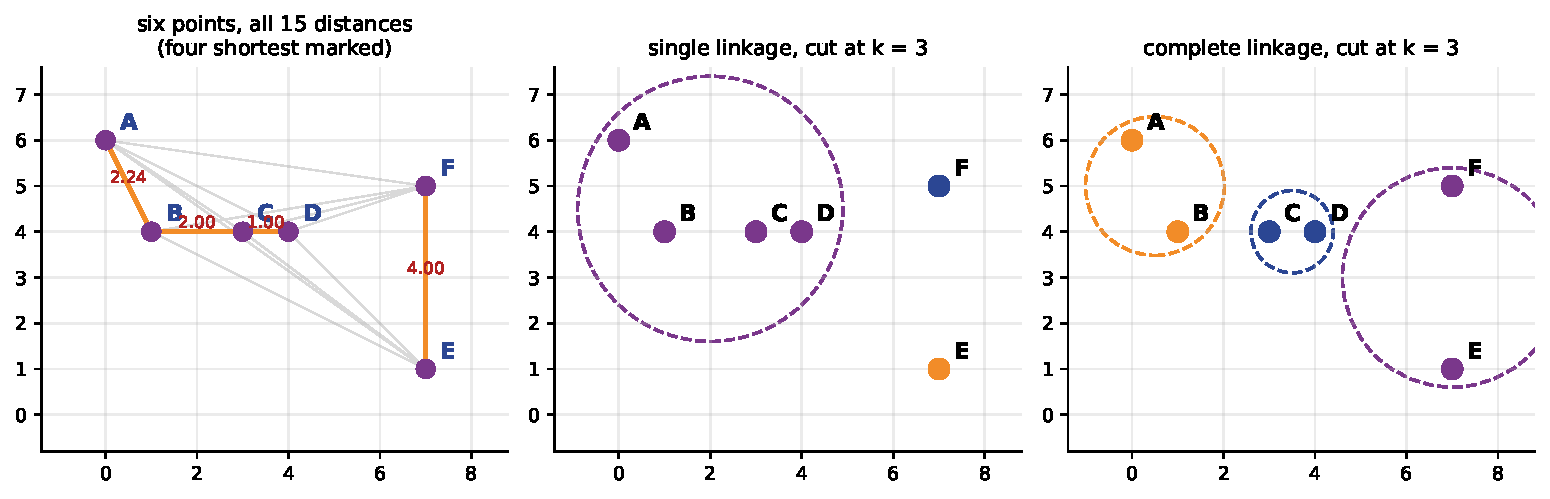
\includegraphics[width=0.99\textwidth]{points.pdf}
  \end{center}
  \vspace{-0.3em}
  \begin{center}\small
    $A(0,6)\quad B(1,4)\quad C(3,4)\quad D(4,4)\quad E(7,1)\quad F(7,5)$
    \\[0.2em]
    Chosen so that all \textbf{fifteen} pairwise distances are distinct --- no
    ties to argue about.
  \end{center}
\end{frame}

\begin{frame}[fragile,shrink=6]{By hand: the initial proximity matrix}
\begin{outblk}
                 A       B       C       D       E       F
A               --  2.2361  3.6056  4.4721  8.6023  7.0711
B           2.2361      --  2.0000  3.0000  6.7082  6.0828
C           3.6056  2.0000      --  1.0000  5.0000  4.1231
D           4.4721  3.0000  1.0000      --  4.2426  3.1623
E           8.6023  6.7082  5.0000  4.2426      --  4.0000
F           7.0711  6.0828  4.1231  3.1623  4.0000      --
\end{outblk}
  \vspace{0.2em}
  \begin{columns}[T]
    \begin{column}{0.52\textwidth}
      \begin{block}{Every entry is $\sqrt{\text{small integer}}$}
        \scriptsize
        $\sqrt{1}, \sqrt{4}, \sqrt{5}, \sqrt{9}, \sqrt{10}, \sqrt{13},
         \sqrt{16}, \sqrt{17}, \sqrt{18}, \sqrt{20}, \sqrt{25}, \sqrt{37},
         \sqrt{45}, \sqrt{50}, \sqrt{74}$ --- integer $\Delta x$ and
        $\Delta y$, so every distance is checkable in your head:
        $d(A,E) = \sqrt{7^2 + 5^2} = \sqrt{74} = 8.6023$.
      \end{block}
    \end{column}
    \begin{column}{0.45\textwidth}
      \begin{exampleblock}{Two numbers to remember}
        Smallest: $d(C,D) = 1.0000$.\\
        Largest: $d(A,E) = 8.6023$.

        \medskip
        Both will turn up as merge heights before the lecture is over.
      \end{exampleblock}
    \end{column}
  \end{columns}
\end{frame}

% =====================================================================
\section[Single linkage]{Single linkage, by hand}
\label{sec:single}

\begin{frame}{Single linkage: nearest neighbour}
  \begin{exampleblock}{}
    \centering\large
    $d_{\text{single}}(A,B) = \displaystyle\min_{a \in A,\ b \in B} d(a,b)$
  \end{exampleblock}
  \begin{columns}[T]
    \begin{column}{0.48\textwidth}
      \begin{block}{The update rule}
        \[
          d(A \cup B,\ K) = \min\bigl(d(A,K),\ d(B,K)\bigr)
        \]
        The new row of the matrix is the \textbf{element-wise minimum} of the
        two old rows.
      \end{block}
    \end{column}
    \begin{column}{0.48\textwidth}
      \begin{alertblock}{No arithmetic at all}
        Nothing is recomputed from the raw points. You look at two numbers and
        keep the smaller one. This is why six points take four minutes with a
        pen --- and why you will be asked to do it.
      \end{alertblock}
    \end{column}
  \end{columns}
\end{frame}

\begin{frame}{Predict first \#1 --- which pair merges first?}
  \begin{alertblock}{Commit to an answer}
    Six singleton clusters. Look at the matrix on the previous slide.

    \medskip
    \centering\large
    Which pair merges first, and does the linkage rule matter?
  \end{alertblock}
  \onslide<2->{
  \begin{exampleblock}{}
    \centering\large
    $\{C\} + \{D\}$ at height $\mathbf{1.0000}$ --- and \textbf{no}, the rule
    does not matter.
  \end{exampleblock}
  \begin{center}\small
    With all clusters singletons, every linkage rule reduces to the same
    thing: $\min$, $\max$ and mean over a set of \emph{one} cross distance are
    all that one distance. \textbf{The first merge is always the smallest
    entry of the original matrix, whichever linkage you chose.} The
    linkages only begin to differ at step 2.
  \end{center}}
\end{frame}

\begin{frame}[fragile]{By hand, step 1: merge $C$ and $D$}
  \begin{center}\small
  New row $=$ element-wise \textbf{minimum} of the $C$ and $D$ rows:\\
  $\min(3.6056,\ 4.4721) = 3.6056$ against $A$; \quad
  $\min(2,\ 3) = 2$ against $B$; \quad
  $\min(5.0000,\ 4.2426) = 4.2426$ against $E$; \quad
  $\min(4.1231,\ 3.1623) = 3.1623$ against $F$.
  \end{center}
\begin{outblk}
                   A         B         E         F        CD
A                 --    2.2361    8.6023    7.0711    3.6056
B             2.2361        --    6.7082    6.0828    2.0000   <-- smallest
E             8.6023    6.7082        --    4.0000    4.2426
F             7.0711    6.0828    4.0000        --    3.1623
CD            3.6056    2.0000    4.2426    3.1623        --
\end{outblk}
  \begin{center}\small
    Five clusters left. The matrix has shrunk by one row and one column.
  \end{center}
\end{frame}

\begin{frame}{Predict first \#2 --- where does $B$ go?}
  \begin{alertblock}{Commit before the matrix is updated}
    $B$ is $2.2361$ from $A$. $B$ is $2.0000$ from $C$ and $3.0000$ from $D$.

    \medskip
    \centering\large
    Does $B$ pair up with $A$, or join $\{C,D\}$? And what if the rule were
    $\max$ instead of $\min$?
  \end{alertblock}
  \onslide<2->{
  \begin{exampleblock}{}
    \centering
    Under $\min$: $d(B, CD) = \min(2, 3) = \mathbf{2.0000} < 2.2361$, so
    \textbf{$B$ joins $\{C,D\}$}.\\[0.3em]
    Under $\max$: $d(B, CD) = \max(2, 3) = \mathbf{3.0000} > 2.2361$, so
    \textbf{$B$ pairs with $A$}.
  \end{exampleblock}
  \begin{center}\small
    \textbf{This one number decides the entire rest of the run.} Two linkages,
    two trees, from the choice between $2.0000$ and $3.0000$ on the same
    two original distances.
  \end{center}}
\end{frame}

\begin{frame}[fragile,shrink=4]{By hand, steps 2 and 3}
  \begin{columns}[T]
    \begin{column}{0.5\textwidth}
      \begin{center}\small\textbf{Step 2: merge $B$ with $CD$ at $2.0000$}\end{center}
\begin{outblk}
                   A         E         F       BCD
A                 --    8.6023    7.0711    2.2361
E             8.6023        --    4.0000    4.2426
F             7.0711    4.0000        --    3.1623
BCD           2.2361    4.2426    3.1623        --
\end{outblk}
    \end{column}
    \begin{column}{0.48\textwidth}
      \begin{center}\small\textbf{Step 3: merge $A$ with $BCD$ at $2.2361$}\end{center}
\begin{outblk}
                   E         F      ABCD
E                 --    4.0000    4.2426
F             4.0000        --    3.1623
ABCD          4.2426    3.1623        --
\end{outblk}
    \end{column}
  \end{columns}
  \vspace{0.4em}
  \begin{alertblock}{Notice what is happening}
    Step 1 attached a point. Step 2 attached a point. Step 3 attached a point.
    One cluster is eating the data one object at a time --- and the next slide
    shows it keep going.
  \end{alertblock}
\end{frame}

\begin{frame}[fragile,shrink=4]{By hand, steps 4 and 5 --- and the answer}
  \begin{columns}[T]
    \begin{column}{0.49\textwidth}
      \begin{center}\small\textbf{Step 4: $F$ joins at $3.1623$}\end{center}
\begin{outblk}
                   E     FABCD
E                 --    4.0000
FABCD         4.0000        --
\end{outblk}
      \begin{center}\scriptsize
        $d(F, ABCD) = 3.1623 < d(E,F) = 4.0000$, so $F$ abandons $E$.
      \end{center}
    \end{column}
    \begin{column}{0.49\textwidth}
      \begin{center}\small\textbf{Step 5: $E$ joins at $4.0000$. Done.}\end{center}
      \begin{exampleblock}{Merge heights, in order}
        \centering\large
        $1.0000,\ 2.0000,\ 2.2361,\ 3.1623,\ 4.0000$
      \end{exampleblock}
    \end{column}
  \end{columns}
  \vspace{0.3em}
  \begin{alertblock}{All five merges attached a single point to one growing cluster}
    \centering
    That behaviour has a name: \textbf{chaining}. Single linkage grows a
    cluster by absorbing whatever is nearest to \emph{anything} already
    inside, so clusters extend along paths of close neighbours. Hold that
    thought --- it is both the method's superpower and its catastrophe.
  \end{alertblock}
\end{frame}

% =====================================================================
\section[Complete linkage]{Complete linkage, on the same points}
\label{sec:complete}

\begin{frame}[shrink=4]{Complete linkage: farthest neighbour}
  \begin{exampleblock}{}
    \centering\large
    $d_{\text{complete}}(A,B) = \displaystyle\max_{a \in A,\ b \in B} d(a,b)$
    \qquad
    $d(A \cup B, K) = \max\bigl(d(A,K),\ d(B,K)\bigr)$
  \end{exampleblock}
  \begin{columns}[T]
    \begin{column}{0.48\textwidth}
      \begin{block}{What it insists on}
        Merging is only cheap if \emph{every} member of one cluster is close
        to \emph{every} member of the other. One distant pair vetoes the
        merge.
      \end{block}
    \end{column}
    \begin{column}{0.48\textwidth}
      \begin{alertblock}{The height has a meaning}
        The height at which a cluster is formed is exactly its
        \textbf{diameter} --- the largest distance between any two of its
        members. That is a genuinely interpretable number, which single
        linkage heights are not.
      \end{alertblock}
    \end{column}
  \end{columns}
\end{frame}

\begin{frame}[fragile,shrink=5]{By hand, complete linkage: steps 1 and 2}
  \begin{columns}[T]
    \begin{column}{0.52\textwidth}
      \begin{center}\small\textbf{Step 1: $C{+}D$ at $1.0000$; new row $= \max$}\end{center}
\begin{outblk}
                   A         B         E         F        CD
A                 --    2.2361    8.6023    7.0711    4.4721
B             2.2361        --    6.7082    6.0828    3.0000
E             8.6023    6.7082        --    4.0000    5.0000
F             7.0711    6.0828    4.0000        --    4.1231
CD            4.4721    3.0000    5.0000    4.1231        --
\end{outblk}
    \end{column}
    \begin{column}{0.46\textwidth}
      \begin{center}\small\textbf{Step 2: $A{+}B$ at $2.2361$}\end{center}
\begin{outblk}
                   E         F        CD        AB
E                 --    4.0000    5.0000    8.6023
F             4.0000        --    4.1231    7.0711
CD            5.0000    4.1231        --    4.4721
AB            8.6023    7.0711    4.4721        --
\end{outblk}
    \end{column}
  \end{columns}
  \vspace{0.3em}
  \begin{center}\small
    Compare the step-1 matrix with the single-linkage one: four entries
    changed and every one of them \textbf{grew}. $d(B,CD)$ went from $2.0000$
    to $3.0000$, and the run turned.
  \end{center}
\end{frame}

\begin{frame}[fragile,shrink=4]{By hand, complete linkage: steps 3, 4, 5}
  \begin{columns}[T]
    \begin{column}{0.46\textwidth}
      \begin{center}\small\textbf{Step 3: $E{+}F$ at $4.0000$}\end{center}
\begin{outblk}
                  CD        AB        EF
CD                --    4.4721    5.0000
AB            4.4721        --    8.6023
EF            5.0000    8.6023        --
\end{outblk}
      \begin{center}\small\textbf{Step 4: $CD{+}AB$ at $4.4721$}\end{center}
\begin{outblk}
                  EF      CDAB
EF                --    8.6023
CDAB          8.6023        --
\end{outblk}
    \end{column}
    \begin{column}{0.52\textwidth}
      \begin{exampleblock}{Step 5, and the heights}
        Merge at $8.6023 = d(A,E)$ --- the largest distance in the data, which
        is the diameter of the whole set.
        \medskip
        \centering\large
        $1.0000,\ 2.2361,\ 4.0000,\ 4.4721,\ 8.6023$
      \end{exampleblock}
      \begin{alertblock}{Check the intermediate numbers}
        $4.4721 = d(A,D)$, the \emph{largest} of the four cross distances
        between $\{A,B\}$ and $\{C,D\}$: $\{2, 3, 3.6056, 4.4721\}$. Complete
        linkage always reports the worst pair.
      \end{alertblock}
    \end{column}
  \end{columns}
\end{frame}

\begin{frame}[fragile,shrink=6]{The two runs, side by side}
\begin{outblk}
step  single-linkage merge            height   complete-linkage merge          height
  1   {C} + {D}                       1.0000   {C} + {D}                       1.0000
  2   {B} + {CD}                      2.0000   {A} + {B}                       2.2361
  3   {A} + {BCD}                     2.2361   {E} + {F}                       4.0000
  4   {F} + {ABCD}                    3.1623   {CD} + {AB}                     4.4721
  5   {E} + {FABCD}                   4.0000   {EF} + {CDAB}                   8.6023
\end{outblk}
  \vspace{0.2em}
  \begin{columns}[T]
    \begin{column}{0.49\textwidth}
      \begin{block}{They agree only at step 1}
        After that, nothing in common: not the pairs, not the heights, not the
        shape.
      \end{block}
    \end{column}
    \begin{column}{0.49\textwidth}
      \begin{alertblock}{Complete heights $\ge$ single heights}
        A maximum over a set cannot be below its minimum. So a complete-linkage
        tree is stretched vertically. \textbf{Never compare a height from one
        linkage with a height from another.}
      \end{alertblock}
    \end{column}
  \end{columns}
\end{frame}

\begin{frame}[shrink=4]{Drawn: the two dendrograms}
  \begin{center}
    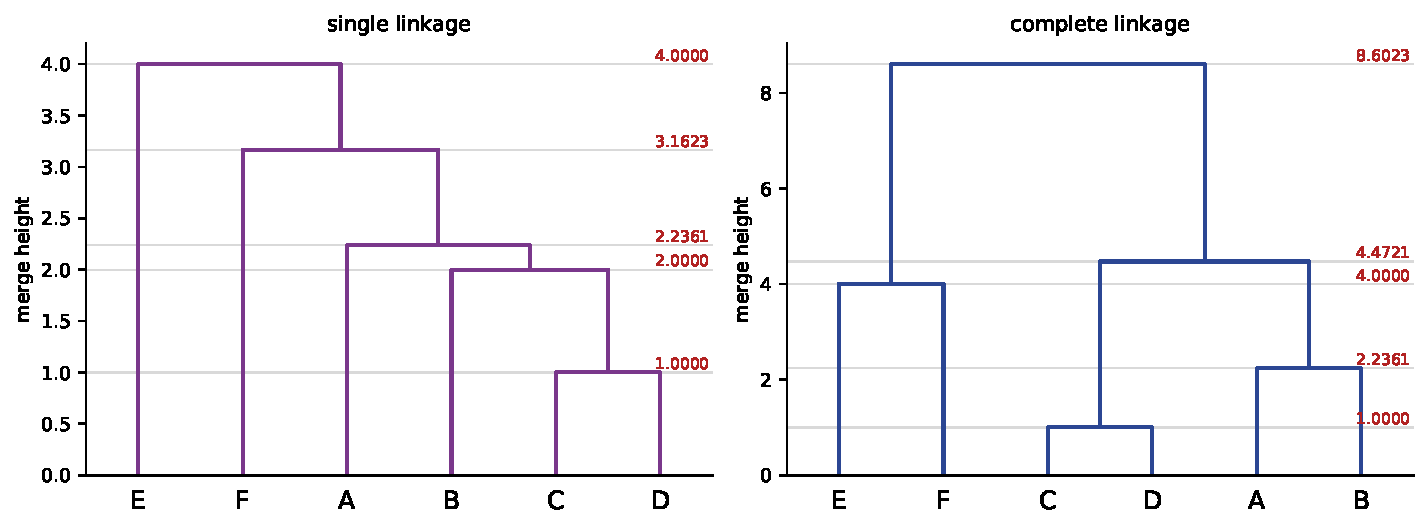
\includegraphics[width=0.88\textwidth]{dendro6.pdf}
  \end{center}
  \vspace{-0.4em}
  \begin{center}\small
    Left, single linkage: a \textbf{staircase}, one point per step. Right,
    complete linkage: three pairs, then two groups, then the root. Same six
    points. Note the vertical scales differ by a factor of two --- and note
    that single linkage draws $E$ and $F$ adjacent although they are the
    \emph{last} two things joined.
  \end{center}
\end{frame}

\begin{frame}[fragile]{The flat clusterings, and the code behind them}
\begin{lstlisting}[basicstyle=\ttfamily\scriptsize]
for k in (2, 3, 4):
    print(k, fcluster(linkage(P6, "single"),   k, "maxclust"),
             fcluster(linkage(P6, "complete"), k, "maxclust"))
\end{lstlisting}
\begin{outblk}
k = 2   single  : {ABCDF} {E}          complete: {EF} {ABCD}
k = 3   single  : {ABCD} {F} {E}       complete: {EF} {CD} {AB}
k = 4   single  : {BCD} {A} {F} {E}    complete: {E} {F} {CD} {AB}
\end{outblk}
  \vspace{0.2em}
  \begin{alertblock}{And the hand run is exact}
    \centering
    \texttt{merge heights in order: 1.0000, 2.0000, 2.2361, 3.1623, 4.0000}\\
    \texttt{scipy heights\ \ \ \ \ \ \ \ \ \ : 1.0000, 2.0000, 2.2361, 3.1623, 4.0000}\\
    \texttt{match to 1e-12: True}
  \end{alertblock}
\end{frame}

\begin{frame}[shrink=4]{One warning before we generalise: ties}
  \begin{alertblock}{These six points were chosen to have no ties}
    All fifteen distances differ. Real data --- integer grids, duplicated
    rows, rounded measurements --- has ties all the time.
  \end{alertblock}
  \begin{columns}[T]
    \begin{column}{0.49\textwidth}
      \begin{block}{What happens then}
        The merge order becomes
        \textbf{implementation-dependent}. SciPy's documentation says so in as
        many words. Two correct programs can return two different trees from
        the same matrix.
      \end{block}
    \end{column}
    \begin{column}{0.49\textwidth}
      \begin{exampleblock}{What to do}
        In an examination: say which tie-break you used and carry on.\\[0.3em]
        In the lab: if the tree changes when you change library version, check
        for ties \emph{before} assuming you have a bug.
      \end{exampleblock}
    \end{column}
  \end{columns}
\end{frame}

% =====================================================================
\section[Five linkages]{The distance between two clusters}
\label{sec:linkage}

\begin{frame}[shrink=10]{Five answers to the one question}
  With $n_A$, $n_B$ the cluster sizes and $c_A$, $c_B$ the centroids:
  \begin{align*}
    d_{\text{single}}(A,B)   &= \min_{a,b} d(a,b)
      &&\text{nearest neighbour}\\
    d_{\text{complete}}(A,B) &= \max_{a,b} d(a,b)
      &&\text{farthest neighbour}\\
    d_{\text{average}}(A,B)  &= \tfrac{1}{n_A n_B}\textstyle\sum_{a}\sum_{b} d(a,b)
      &&\text{UPGMA}\\
    d_{\text{centroid}}(A,B) &= \lVert c_A - c_B \rVert_2
      &&\text{UPGMC}\\
    d_{\text{ward}}(A,B)     &= \sqrt{\tfrac{2 n_A n_B}{n_A + n_B}}\,
                                \lVert c_A - c_B \rVert_2
      &&\text{minimum variance}
  \end{align*}
  \vspace{-0.4em}
  \begin{center}\small
    \textbf{First three: any dissimilarity} --- they only look up entries of
    $D$, so edit distances, cosine and Jaccard are all fine.\\
    \textbf{Last two: Euclidean only} --- a centroid needs a vector space, and
    SciPy will not stop you handing \texttt{ward} a cosine matrix.
  \end{center}
\end{frame}

\begin{frame}{Drawn: what each rule actually measures}
  \begin{center}
    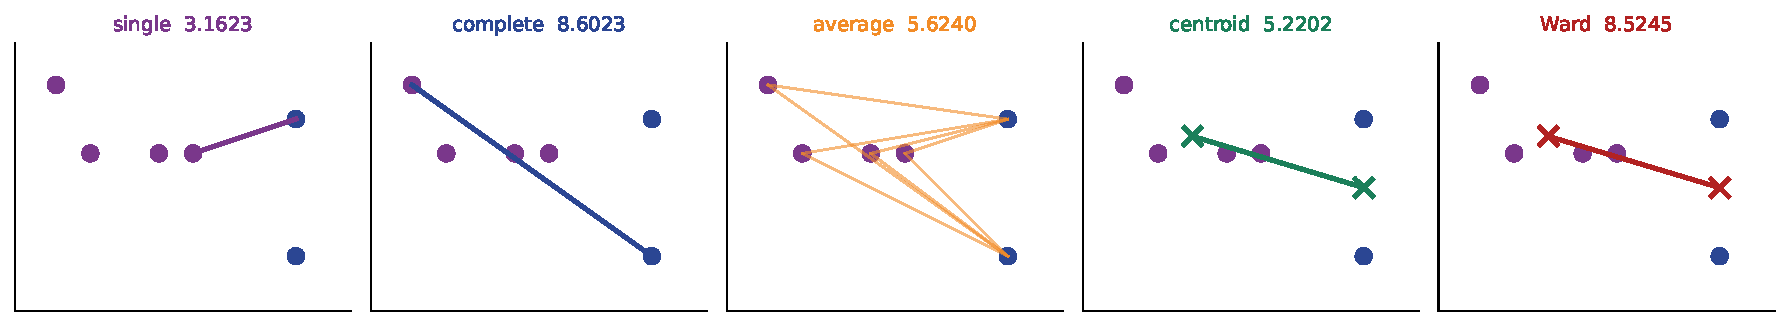
\includegraphics[width=\textwidth]{whatmeasured.pdf}
  \end{center}
  \vspace{-0.2em}
  \begin{center}\small
    The same two clusters, $\{A,B,C,D\}$ against $\{E,F\}$, measured five
    ways. Single takes one of the eight cross distances; complete takes
    another; average takes all eight; centroid and Ward work from the crosses.
  \end{center}
\end{frame}

\begin{frame}[fragile,shrink=6]{By hand: all five, for $\{A,B,C,D\}$ against $\{E,F\}$}
  \begin{center}\small
    Eight cross distances, from the original matrix:
    $\{8.6023,\ 7.0711,\ 6.7082,\ 6.0828,\ 5.0000,\ 4.1231,\ 4.2426,\ 3.1623\}$
  \end{center}
\begin{outblk}
  single   min          = 3.1623                       (the pair D,F)
  complete max          = 8.6023                       (the pair A,E)
  average  mean         = 44.9924 / 8 = 5.6240
  centroid ||cA - cB||  = 5.2202   cA = (2.0000, 4.5000)  cB = (7.0000, 3.0000)
  ward     sqrt(2*nA*nB/(nA+nB))*||cA-cB|| = sqrt(2.6667)*5.2202 = 8.5245
\end{outblk}
  \vspace{0.2em}
  \begin{columns}[T]
    \begin{column}{0.49\textwidth}
      \begin{block}{The centroids, by hand}
        \small
        $c_A = \frac14(0{+}1{+}3{+}4,\ 6{+}4{+}4{+}4) = (2.0,\ 4.5)$\\
        $c_B = \frac12(7{+}7,\ 1{+}5) = (7.0,\ 3.0)$\\
        $\lVert c_A - c_B\rVert = \sqrt{5^2 + 1.5^2} = \sqrt{27.25} = 5.2202$
      \end{block}
    \end{column}
    \begin{column}{0.49\textwidth}
      \begin{alertblock}{}
        \centering
        Five numbers between $3.16$ and $8.60$, all correctly describing the
        distance between the \emph{same} two clusters.
      \end{alertblock}
    \end{column}
  \end{columns}
\end{frame}

\begin{frame}[shrink=10]{Where Ward's formula comes from}
  \begin{block}{The only one of the five with an objective}
    \small Within-cluster sum of squares
    $\mathrm{ESS}(A) = \sum_{a \in A}\lVert a - c_A\rVert^2$: zero at the
    singleton level, maximal at the root. \textbf{Ward merges the pair that
    increases the total by the least.}
  \end{block}
  \begin{exampleblock}{}
    \centering\large
    $\Delta(A,B) = \mathrm{ESS}(A \cup B) - \mathrm{ESS}(A) - \mathrm{ESS}(B)
     = \dfrac{n_A n_B}{n_A + n_B}\lVert c_A - c_B\rVert^2$
  \end{exampleblock}
  \begin{columns}[T]
    \begin{column}{0.49\textwidth}
      \begin{block}{SciPy reports $\sqrt{2\Delta}$}
        \small
        $\Delta = \frac{4 \cdot 2}{6}\times 27.25 = 36.3333$, and
        $\sqrt{2 \times 36.3333} = \mathbf{8.5245}$ --- the number in the
        block above. The factor of $2$ makes the height equal $d(a,b)$ for two
        singletons.
      \end{block}
    \end{column}
    \begin{column}{0.49\textwidth}
      \begin{alertblock}{One sentence to remember}
        \small Ward is $k$-means' objective run greedily bottom-up: compact,
        similarly sized, roughly spherical clusters. The sensible default on
        numeric data.
      \end{alertblock}
    \end{column}
  \end{columns}
\end{frame}

% =====================================================================
\section[Lance--Williams]{One formula for all five}
\label{sec:lw}

\begin{frame}[shrink=14]{The Lance--Williams recurrence (1967)}
  \begin{exampleblock}{}
    \centering\large
    $d(A \cup B,\ K) = \alpha_A d(A,K) + \alpha_B d(B,K) + \beta\, d(A,B)
      + \gamma\,\bigl|d(A,K) - d(B,K)\bigr|$
  \end{exampleblock}
  \begin{center}\small
  \begin{tabular}{lllll}
    \toprule
    method & $\alpha_A$ & $\alpha_B$ & $\beta$ & $\gamma$ \\
    \midrule
    single   & $1/2$ & $1/2$ & $0$ & $-1/2$ \\
    complete & $1/2$ & $1/2$ & $0$ & $+1/2$ \\
    average  & $n_A/(n_A{+}n_B)$ & $n_B/(n_A{+}n_B)$ & $0$ & $0$ \\
    centroid & $n_A/(n_A{+}n_B)$ & $n_B/(n_A{+}n_B)$ &
               $-n_A n_B/(n_A{+}n_B)^2$ & $0$ \\
    Ward     & $(n_A{+}n_K)/T$ & $(n_B{+}n_K)/T$ & $-n_K/T$ & $0$ \\
    \bottomrule
  \end{tabular}
  \end{center}
  \begin{columns}[T]
    \begin{column}{0.49\textwidth}
      \begin{block}{}
        \small $T = n_A + n_B + n_K$. \textbf{Centroid and Ward act on
        squared distances}; take the square root at the end.
      \end{block}
    \end{column}
    \begin{column}{0.49\textwidth}
      \begin{alertblock}{}
        \small The new distance depends only on \textbf{three numbers already
        in the matrix}. The raw points are never revisited.
      \end{alertblock}
    \end{column}
  \end{columns}
\end{frame}

\begin{frame}[shrink=3]{By hand: $\min$ and $\max$ fall out of the formula}
  \begin{block}{Put $\alpha_A = \alpha_B = 1/2$, $\beta = 0$, $\gamma = -1/2$, and write $u = d(A,K)$, $v = d(B,K)$}
    \[
      \tfrac12 u + \tfrac12 v - \tfrac12|u - v|
      \;=\; \frac{u + v - |u-v|}{2} \;=\; \min(u, v),
    \]
    because if $u \le v$ then $|u-v| = v - u$ and the expression is
    $(u + v - v + u)/2 = u$. Flip the sign of $\gamma$ and the same algebra
    gives $\max(u,v)$. \ensuremath{\square}
  \end{block}
  \begin{alertblock}{Why this matters practically}
    \centering
    One merge loop, four constants. That is why a single $O(n^2)$-memory
    implementation serves every linkage --- and why the proximity matrix is
    the only thing HAC ever has to keep.
  \end{alertblock}
\end{frame}

\begin{frame}[fragile,shrink=5]{In code: the recurrence reproduces SciPy}
\begin{lstlisting}[basicstyle=\ttfamily\scriptsize]
for method in ("single", "complete", "average", "centroid", "ward"):
    h = lance_williams(P6, method)      # uses only the recurrence
    print(method, h, linkage(P6, method=method)[:, 2])
\end{lstlisting}
\begin{outblk}
  single    LW 1.0000 2.0000 2.2361 3.1623 4.0000 | scipy same | match True
  complete  LW 1.0000 2.2361 4.0000 4.4721 8.6023 | scipy same | match True
  average   LW 1.0000 2.2361 3.2694 4.0000 5.6240 | scipy same | match True
  centroid  LW 1.0000 2.2361 3.1623 4.0000 5.2202 | scipy same | match True
  ward      LW 1.0000 2.2361 4.0000 4.4721 8.5245 | scipy same | match True
\end{outblk}
  \begin{center}\small
    The last average-linkage height, $\mathbf{5.6240}$, is the mean of the
    eight cross distances we computed by hand --- reached by the recurrence
    without ever looking at a coordinate. Centroid's $5.2202$ and Ward's
    $8.5245$ are likewise the two numbers from the worked example.
  \end{center}
\end{frame}

\begin{frame}[fragile]{All five on the six points, and their $k=2$ answers}
\begin{outblk}
  single    C+D@1.000  B+CD@2.000  A+BCD@2.236  F+ABCD@3.162  E+FABCD@4.000
  complete  C+D@1.000  A+B@2.236   E+F@4.000    CD+AB@4.472   EF+CDAB@8.602
  average   C+D@1.000  A+B@2.236   CD+AB@3.269  E+F@4.000     CDAB+EF@5.624
  centroid  C+D@1.000  A+B@2.236   CD+AB@3.162  E+F@4.000     CDAB+EF@5.220
  ward      C+D@1.000  A+B@2.236   E+F@4.000    CD+AB@4.472   EF+CDAB@8.524
\end{outblk}
  \vspace{0.3em}
  \begin{exampleblock}{}
    \centering
    Four of the five recover $\{A,B,C,D\}$ and $\{E,F\}$ at $k = 2$.\\
    \textbf{Only single linkage does not} --- it gives $\{A,B,C,D,F\}$ and the
    lone point $\{E\}$.
  \end{exampleblock}
\end{frame}

% =====================================================================
\section[Shape and chaining]{What linkage does to cluster shape}
\label{sec:shape}

\begin{frame}[shrink=6]{Linkage is a belief about shape --- measured}
  \begin{center}
    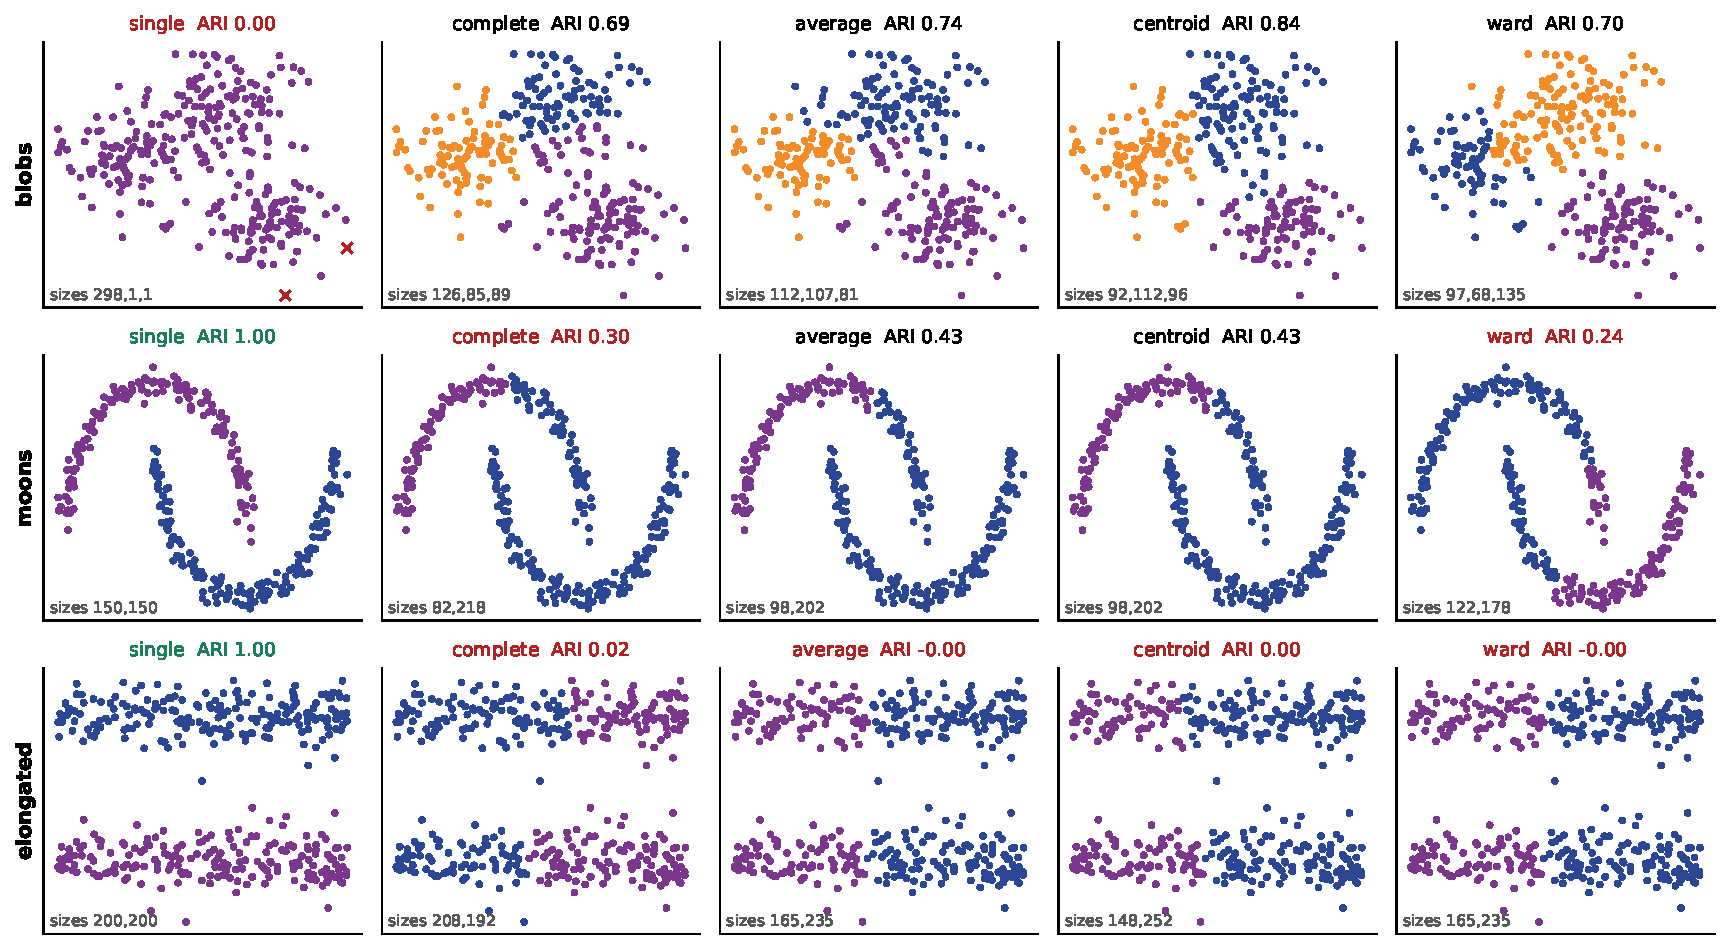
\includegraphics[width=0.66\textwidth]{linkgrid.pdf}
  \end{center}
  \vspace{-0.5em}
  \begin{columns}[T]
    \begin{column}{0.32\textwidth}
      \begin{block}{Single says}
        \centering\textbf{connected}\\[0.2em]
        \scriptsize anything you can walk across in small steps
      \end{block}
    \end{column}
    \begin{column}{0.32\textwidth}
      \begin{block}{Complete says}
        \centering\textbf{small diameter}\\[0.2em]
        \scriptsize a set in which no two members are far apart
      \end{block}
    \end{column}
    \begin{column}{0.32\textwidth}
      \begin{block}{Ward says}
        \centering\textbf{low variance}\\[0.2em]
        \scriptsize a set that is well described by its mean
      \end{block}
    \end{column}
  \end{columns}
  \vspace{0.2em}
  \begin{center}\scriptsize
    Adjusted Rand index against the known truth; red crosses mark clusters of
    three points or fewer. \textbf{Linkage is not a tuning knob} --- choose the
    belief that matches your data.
  \end{center}
\end{frame}

\begin{frame}[fragile,shrink=8]{The numbers behind that grid}
\begin{outblk}
data        linkage      ARI    sizes         data        linkage      ARI    sizes
blobs       single     0.000  298,1,1         moons       single     1.000  150,150
blobs       complete   0.692 126,85,89        moons       complete   0.297   82,218
blobs       average    0.741 112,107,81       moons       average    0.425   98,202
blobs       centroid   0.844  92,112,96       moons       centroid   0.425   98,202
blobs       ward       0.697  97,68,135       moons       ward       0.241  122,178

elongated   single     1.000  200,200         elongated   average   -0.002  165,235
elongated   complete   0.017  208,192         elongated   ward      -0.002  165,235
\end{outblk}
  \vspace{0.2em}
  \begin{columns}[T]
    \begin{column}{0.49\textwidth}
      \begin{exampleblock}{Single linkage is the only one that follows a curve}
        \small ARI $\mathbf{1.000}$ on the moons and on two long bands, where
        everything else is near-random. It walks the arc one neighbour at a
        time; the shape is irrelevant to it.
      \end{exampleblock}
    \end{column}
    \begin{column}{0.49\textwidth}
      \begin{alertblock}{And it collapses on touching blobs}
        \small $\mathbf{298/1/1}$, ARI $\mathbf{0.000}$. The blobs touch, so
        the chain runs straight through; the only merges left for the top of
        the tree are the two most isolated points.
      \end{alertblock}
    \end{column}
  \end{columns}
\end{frame}

\begin{frame}[shrink=7]{And complete linkage and Ward break long clusters}
  \begin{columns}[T]
    \begin{column}{0.5\textwidth}
      \begin{block}{Look at the bottom row again}
        The truth is two horizontal bands. Complete linkage and Ward return a
        \textbf{left half and a right half}: ARI $0.017$ and $-0.002$.
      \end{block}
      \begin{exampleblock}{They are not confused}
        They are doing their job. A long thin band has enormous diameter and
        enormous variance. A method that minimises either of those genuinely
        prefers two compact halves.
      \end{exampleblock}
    \end{column}
    \begin{column}{0.47\textwidth}
      \begin{alertblock}{The mismatch is between the objective and the data}
        Not inside the algorithm. There is no bug to fix and no parameter to
        tune. If your clusters are long and thin, do not ask a
        variance-minimising method to find them.

        \medskip
        This is the single most useful sentence in the lecture for the lab.
      \end{alertblock}
    \end{column}
  \end{columns}
\end{frame}

\begin{frame}{Predict first \#3 --- twelve points in the gap}
  \begin{alertblock}{Commit to an answer}
    Two clean Gaussian clusters, sixty points each, at $x = 0$ and $x = 8$.
    The nearest point of one to the nearest point of the other is
    $\mathbf{5.5714}$ away. Every linkage separates them perfectly.

    \medskip
    Now scatter \textbf{twelve} noise points in a line across the gap --- ten
    per cent of the data, none of it near either cluster.

    \medskip
    \centering\large
    What does single linkage give at $k = 2$? What do complete and Ward give?
  \end{alertblock}
  \onslide<2->{
  \begin{exampleblock}{}
    \centering\large
    Single: $\mathbf{[131,\ 1]}$, ARI $\mathbf{0.000}$. \qquad
    Complete and Ward: $[70,\ 62]$, ARI $\mathbf{1.000}$.
  \end{exampleblock}}
\end{frame}

\begin{frame}[fragile,shrink=8]{Measured: the chaining collapse}
\begin{outblk}
bridge  linkage    height at which the two true clusters fuse   k = 2 sizes   ARI
   0    single                                   5.571   [60, 60]     1.000
   0    complete                                10.381   [60, 60]     1.000
   0    ward                                    62.573   [60, 60]     1.000
   4    single                                   2.005   [62, 62]     1.000
   8    single                                   0.869   [67, 61]     1.000
  12    single                                   0.565   [131, 1]     0.000
  12    complete                                10.381   [70, 62]     1.000
  12    ward                                    61.146   [70, 62]     1.000
  16    single                                   0.434   [135, 1]     0.000
  16    complete                                10.381   [70, 66]     1.000
\end{outblk}
  \vspace{0.2em}
  \begin{columns}[T]
    \begin{column}{0.49\textwidth}
      \begin{alertblock}{Read the single column downwards}
        \centering
        $5.571 \to 2.005 \to 0.869 \to 0.565 \to 0.434$\\[0.2em]
        \small A factor of ten, from twelve stray points.
      \end{alertblock}
    \end{column}
    \begin{column}{0.49\textwidth}
      \begin{block}{The other two do not move}
        \small Complete fuses at $10.381$ whatever you do --- that is
        $\max_{a,b} d(a,b)$ across the two clusters, and no bridge point can
        reduce a maximum.
      \end{block}
    \end{column}
  \end{columns}
\end{frame}

\begin{frame}{Drawn: the same result}
  \begin{center}
    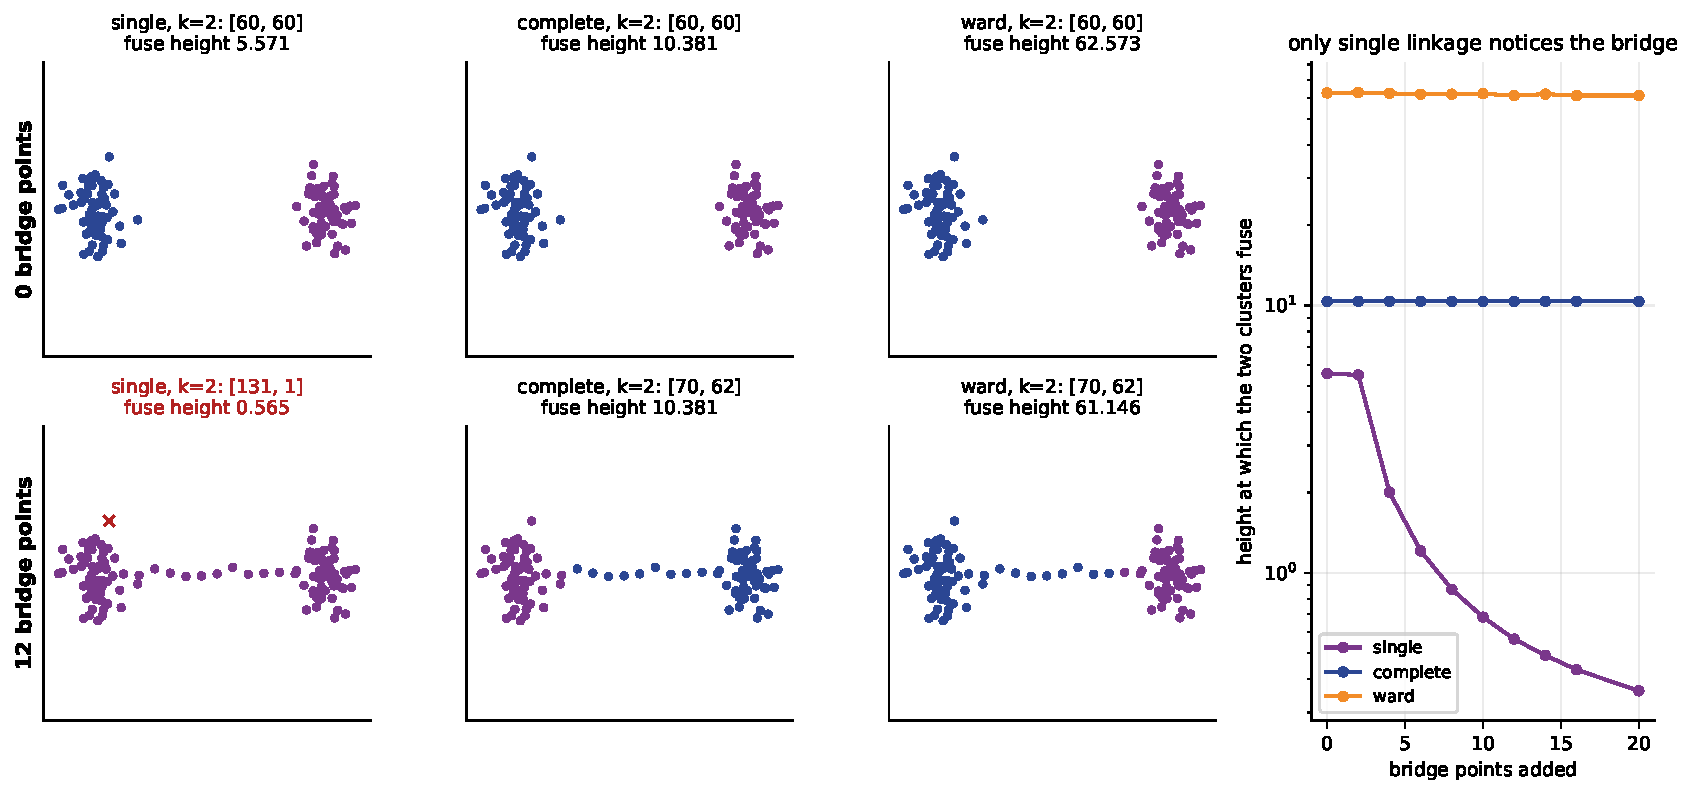
\includegraphics[width=0.74\textwidth]{chaining.pdf}
  \end{center}
  \vspace{-0.4em}
  \begin{center}\scriptsize
    Bottom left: single linkage's ``two clusters'' are $131$ points and the
    red cross. Right: fusion height against bridge size, log scale --- only
    the purple line moves.
  \end{center}
\end{frame}

\begin{frame}[fragile,shrink=5]{Why: single linkage never pays the gap}
\begin{outblk}
  nb  spacing  bottleneck step on the left-bridge-right path  single fuse height
   0      nan                          5.5714               5.5714
   4   2.0000                          2.0021               2.0048
   8   0.8571                          0.8687               0.8687
  12   0.5455                          0.5634               0.5653
  16   0.4000                          0.4242               0.4341
\end{outblk}
  \vspace{0.3em}
  \begin{exampleblock}{}
    \centering
    The fusion height is \textbf{exactly the largest single step along the
    path} left $\to$ bridge $\to$ right --- the bottleneck. Single linkage is
    measuring \emph{connectivity}, and a thin bridge is a connection.
  \end{exampleblock}
  \begin{alertblock}{The examinable version of ``chaining''}
    \centering\small
    The linkage takes a \textbf{minimum} over cross pairs, so \emph{one} short
    link is enough to fuse two clusters --- and a path of noise supplies one.
    A maximum, or a mean over $n_A n_B$ pairs, cannot be dragged down by a
    single pair.
  \end{alertblock}
\end{frame}

% =====================================================================
\section[Inversions]{Centroid linkage can go backwards}
\label{sec:inv}

\begin{frame}{Predict first \#4 --- can a dendrogram go down?}
  \begin{alertblock}{Commit to an answer}
    Every merge height so far has been at least as large as the one before.
    That property --- \textbf{monotonicity} --- is what makes ``cut at height
    $h$'' meaningful.

    \medskip
    \centering\large
    Is a later merge \emph{always} at least as high as an earlier one? If not,
    what is the smallest counterexample?
  \end{alertblock}
  \onslide<2->{
  \begin{exampleblock}{}
    \centering\large
    Single, complete, average and Ward: \textbf{always monotone}.\\
    Centroid: \textbf{no} --- and the counterexample needs
    \textbf{three points}.
  \end{exampleblock}
  \begin{center}\small
    The four monotone methods are \emph{reducible}: if $A$ and $B$ are each at
    least $\delta$ from $K$, so is $A \cup B$. Centroid linkage is not.
  \end{center}}
\end{frame}

\begin{frame}[fragile,shrink=5]{By hand: an inversion on three points}
  \begin{columns}[T]
    \begin{column}{0.52\textwidth}
      \begin{block}{$P_1 = (0,0)$, $P_2 = (1,0)$, $P_3 = (0.48, 0.84)$}
        \small
        $d(P_1,P_2) = 1.0000$, \quad $d(P_1,P_3) = 0.9675$, \quad
        $d(P_2,P_3) = 0.9879$.
        \medskip

        Smallest is $d(P_1,P_3)$: \textbf{merge at $0.9675$}.
        Their centroid is $c = (0.2400,\ 0.4200)$, and
        \[
          \lVert c - P_2\rVert = \sqrt{0.5776 + 0.1764} = \sqrt{0.7540}
          = \mathbf{0.8683}.
        \]
      \end{block}
    \end{column}
    \begin{column}{0.46\textwidth}
\begin{outblk}
scipy centroid heights: 0.9675 0.8683
monotone: False   drop = 0.0991
  single    0.9675 0.9879  monotone True
  complete  0.9675 1.0000  monotone True
  average   0.9675 0.9940  monotone True
  ward      0.9675 1.0027  monotone True
\end{outblk}
    \end{column}
  \end{columns}
  \vspace{0.3em}
  \begin{alertblock}{The geometry, in one sentence}
    \centering
    The centroid of a merged pair lies \emph{between} its two members, so it
    is closer to everything outside than at least one of them was.
    \textbf{Averaging moves you inward.}
  \end{alertblock}
\end{frame}

\begin{frame}[fragile]{Drawn --- and it is not a corner case}
  \begin{columns}[T]
    \begin{column}{0.66\textwidth}
      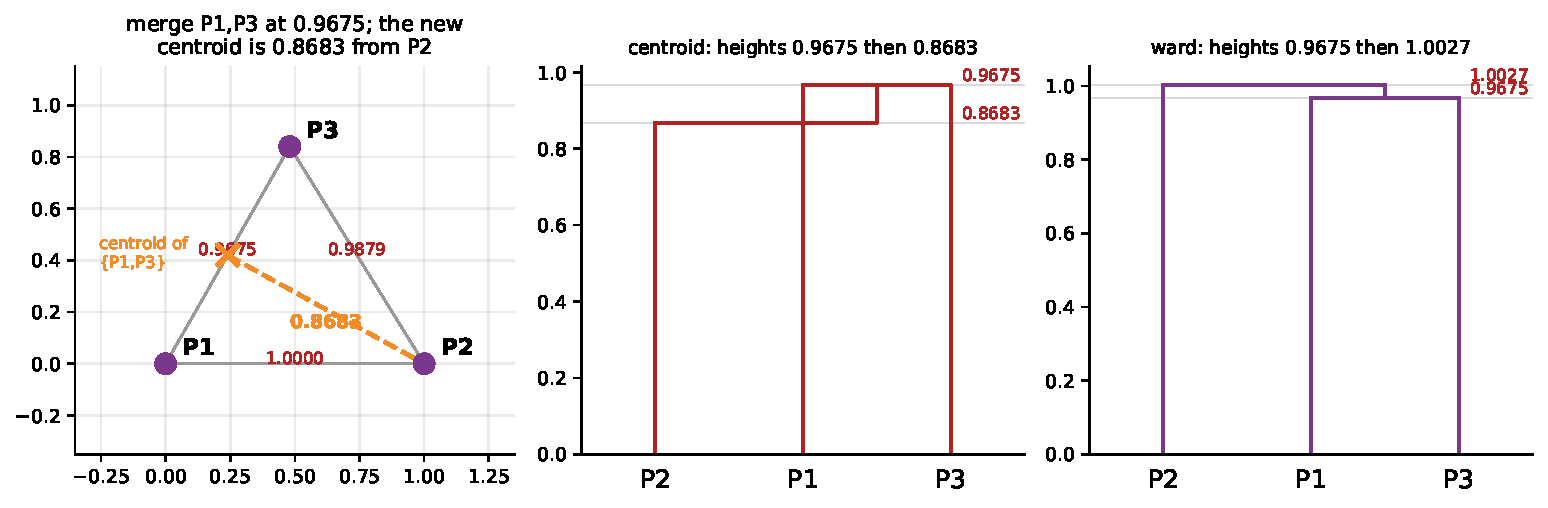
\includegraphics[width=\textwidth]{inversion.pdf}
    \end{column}
    \begin{column}{0.32\textwidth}
\begin{outblk}
 n=5  uniform points:  6.2%
 n=10 uniform points: 22.2%
 n=25 uniform points: 54.5%
 n=50 uniform points: 75.5%
\end{outblk}
      \begin{center}\scriptsize
        Fraction of centroid trees containing at least one inversion,
        400 random point sets each.
      \end{center}
    \end{column}
  \end{columns}
  \vspace{0.2em}
  \begin{alertblock}{What an inversion costs you}
    \centering\small
    ``Cut at height $h$'' stops being well defined: a cluster formed at $0.97$
    can sit \emph{underneath} an edge drawn at $0.87$. Use average linkage
    instead --- it answers almost the same question and is monotone.
  \end{alertblock}
\end{frame}

% =====================================================================
\section[Cutting]{Cutting the dendrogram}
\label{sec:cut}

\begin{frame}[fragile,shrink=4]{A tree is not a clustering. Cut it.}
  \begin{columns}[T]
    \begin{column}{0.46\textwidth}
      \begin{block}{Two ways}
        \small
        \texttt{fcluster(Z, k, "maxclust")} --- by count: stop after $n-k$
        merges.\\[0.4em]
        \texttt{fcluster(Z, t, "distance")} --- by height: cut at $t$, take
        however many components result.
      \end{block}
    \end{column}
    \begin{column}{0.52\textwidth}
\begin{outblk}
  cut at height   4.0 -> 8 clusters
  cut at height   6.0 -> 5 clusters, 20,29,30,45,26
  cut at height   8.0 -> 4 clusters, 49,30,45,26
  cut at height  10.0 -> 3 clusters, 49,30,71
  cut at height  12.0 -> 3 clusters, 49,30,71
  cut at height  16.0 -> 2 clusters, 49,101
\end{outblk}
    \end{column}
  \end{columns}
  \vspace{0.3em}
  \begin{exampleblock}{}
    \centering
    Cutting at $10$ and at $12$ give the same answer, because no merge happens
    in between. \textbf{That gap is the whole basis of the usual advice about
    where to cut.}
  \end{exampleblock}
\end{frame}

\begin{frame}[shrink=9]{Predict first \#5 --- how many clusters are in iris?}
  \begin{alertblock}{Commit to an answer}
    Iris: $150$ flowers, four measurements, standardised, Ward linkage. The
    last eight merge heights are
    \[
      3.95,\ 4.06,\ 4.23,\ 4.24,\ 6.61,\ 8.00,\ 12.64,\ 27.25 .
    \]
    The gap heuristic says: cut where the tree has a long stretch with no
    merges.

    \medskip
    \centering\large
    What $k$ does the heuristic choose --- and iris has three species.
  \end{alertblock}
  \onslide<2->{
  \begin{exampleblock}{}
    \centering\large
    The biggest gap is $27.25 - 12.64 = \mathbf{14.61}$, the very last merge.
    \\ The heuristic says $\mathbf{k = 2}$. Silhouette also says $k = 2$
    ($0.5770$ against $0.4467$).
    \\ ARI against the species is best at $k = 3$ ($0.6153$ against $0.5438$).
  \end{exampleblock}}
\end{frame}

\begin{frame}{Drawn: the tree, the gaps, and the truth}
  \begin{center}
    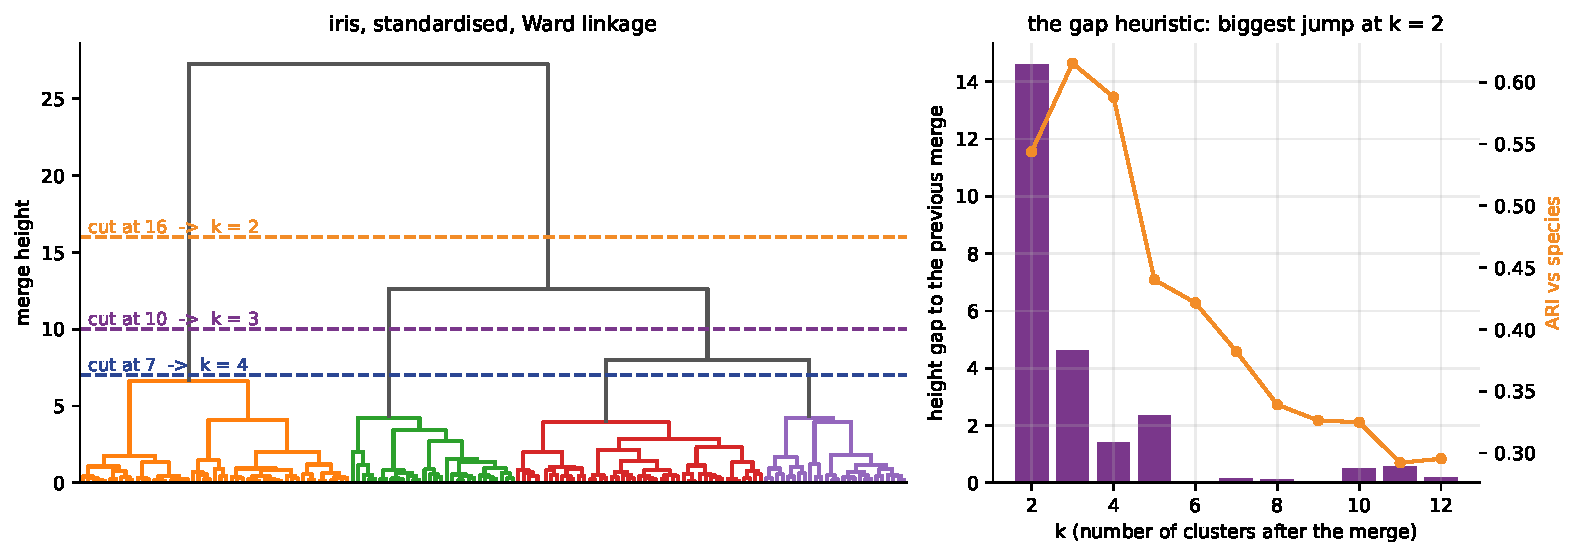
\includegraphics[width=0.97\textwidth]{cutting.pdf}
  \end{center}
  \vspace{-0.4em}
  \begin{center}\scriptsize
    Right-hand panel: the height gap at each $k$ (bars) against ARI with the
    true species (orange). They peak in different places.
  \end{center}
\end{frame}

\begin{frame}[shrink=6]{Be honest about what the gap rule is}
  \begin{alertblock}{It is a heuristic, not a criterion}
    \small It is not wrong on iris --- two species genuinely overlap. But the
    rule \textbf{almost always points at small $k$}: merge heights grow
    super-linearly towards the root, so the last gap is nearly always the
    largest.
  \end{alertblock}
  \begin{columns}[T]
    \begin{column}{0.49\textwidth}
      \begin{block}{What to do instead}
        \small The whole gap profile, not just the maximum. Cross-check with
        silhouette. Check the cluster \emph{sizes} --- ``two clusters'' of
        $149/1$ is outlier-peeling, not structure. Then domain knowledge.
      \end{block}
    \end{column}
    \begin{column}{0.49\textwidth}
      \begin{exampleblock}{The deeper point}
        \small Two unsupervised criteria agreed with each other and disagreed
        with the labels. That is normal. \textbf{The number of clusters in the
        data and the number of classes in the label column are different
        quantities.}
      \end{exampleblock}
    \end{column}
  \end{columns}
\end{frame}

\begin{frame}[fragile,shrink=5]{What the $k = 3$ cut actually did}
  \begin{columns}[T]
    \begin{column}{0.62\textwidth}
      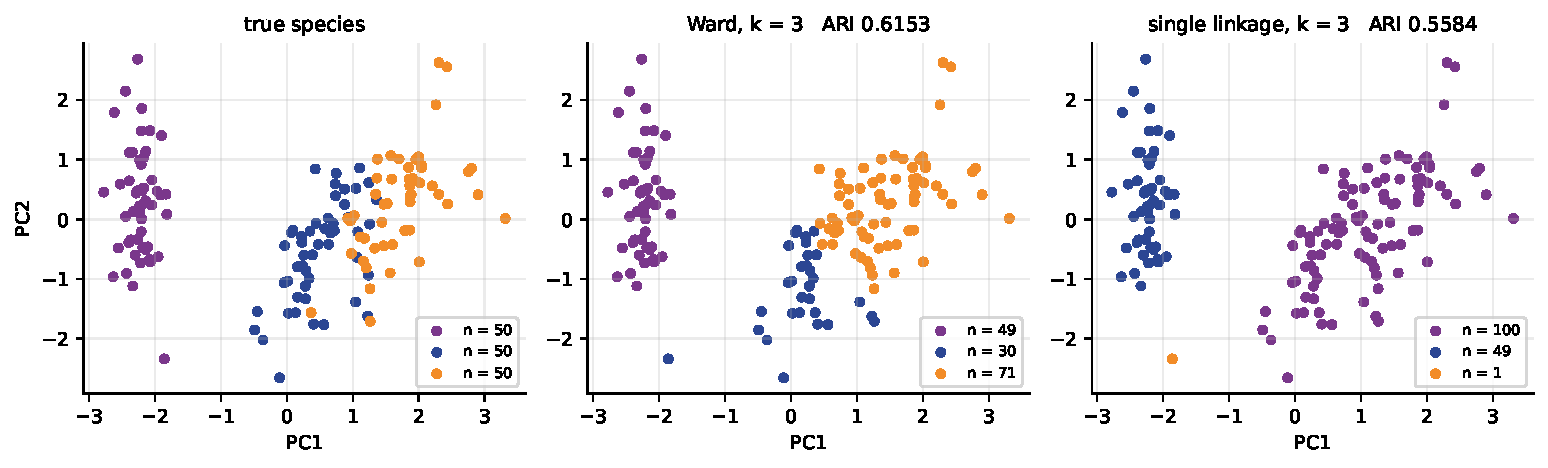
\includegraphics[width=\textwidth]{irispca.pdf}
    \end{column}
    \begin{column}{0.36\textwidth}
\begin{outblk}
           cl 1  cl 2  cl 3
species 0    49     1     0
species 1     0    27    23
species 2     0     2    48
\end{outblk}
      \begin{block}{}
        \small Setosa recovered almost exactly. Versicolor and virginica split
        $27/23$ and $2/48$ --- the boundary is genuinely fuzzy in the
        measurements.
      \end{block}
    \end{column}
  \end{columns}
  \vspace{0.2em}
  \begin{alertblock}{}
    \centering\small
    Right-hand panel: \textbf{single linkage on the identical data} gives
    $100/49/1$ --- one giant cluster and a stray point. Same failure mode as
    the touching blobs.
  \end{alertblock}
\end{frame}

\begin{frame}[fragile,shrink=5]{Two decisions that matter more than the linkage}
  \begin{columns}[T]
    \begin{column}{0.48\textwidth}
      \begin{block}{Scaling}
\begin{outblk}
  raw centimetres     ARI = 0.7312
  standardised        ARI = 0.6153
  one column x100     ARI = 0.2879
\end{outblk}
        \small On iris, standardising made it \textbf{worse}: the four columns
        are already in the same unit, and the larger variance of the petal
        measurements is real signal.
      \end{block}
    \end{column}
    \begin{column}{0.48\textwidth}
      \begin{block}{The dissimilarity itself (wine, average linkage)}
\begin{outblk}
  euclidean     ARI -0.0054   3,174,1
  cityblock     ARI  0.4730  51,126,1
  cosine        ARI  0.7847  68,52,58
  correlation   ARI  0.8224  56,58,64
\end{outblk}
        \small Same linkage, same rows. $-0.0054$ against $0.8224$.
      \end{block}
    \end{column}
  \end{columns}
  \vspace{0.3em}
  \begin{alertblock}{}
    \centering
    Both of these change the answer more than the choice of linkage does. The
    previous lecture was about exactly this, and \textbf{this is where it
    pays}.
  \end{alertblock}
\end{frame}

% =====================================================================
\section[Time and space]{Time and space requirements}
\label{sec:cost}

\begin{frame}{Predict first \#6 --- can you cluster $100{,}000$ rows?}
  \begin{alertblock}{Commit to a number}
    You have $100{,}000$ customer records and a laptop with $16$\,GiB of
    memory. You want a dendrogram.

    \medskip
    \centering\large
    How much memory does the proximity matrix alone need?
  \end{alertblock}
  \onslide<2->{
  \begin{exampleblock}{}
    \centering\large
    $\dfrac{100000 \times 99999}{2} \times 8\ \text{bytes}
     = 4{,}999{,}950{,}000 \times 8 = \mathbf{37.3\ \text{GiB}}$
  \end{exampleblock}
  \begin{center}\small
    And that is the \emph{compact} triangular form, before the algorithm
    allocates anything else. \textbf{This one number is why hierarchical
    clustering does not appear in production pipelines over large data.}
  \end{center}}
\end{frame}

\begin{frame}[fragile,shrink=6]{Space: $O(n^2)$, and it is the binding constraint}
\begin{outblk}
        n        pairs n(n-1)/2   condensed float64      full square
      100                4,950           38.7 KiB         78.1 KiB
    1,000              499,500            3.8 MiB          7.6 MiB
   10,000           49,995,000          381.4 MiB        762.9 MiB
   50,000        1,249,975,000            9.3 GiB         18.6 GiB
  100,000        4,999,950,000           37.3 GiB         74.5 GiB
1,000,000      499,999,500,000            3.6 TiB          7.3 TiB
measured: pdist on 10,000 points returns float64 of shape (49995000,) -> 381.4 MiB
\end{outblk}
  \vspace{0.2em}
  \begin{columns}[T]
    \begin{column}{0.49\textwidth}
      \begin{block}{Turn it around}
        \small
        $8$\,GiB of memory $\Rightarrow n < 46{,}341$.\\
        $64$\,GiB of memory $\Rightarrow n < 131{,}072$.\\
        And that assumes nothing else is resident.
      \end{block}
    \end{column}
    \begin{column}{0.49\textwidth}
      \begin{alertblock}{No algorithm can rescue this}
        \small The memory is in the \emph{input}, not in the merge loop.
        \texttt{float32} buys you a factor of $\sqrt{2}$ in $n$ and changes
        nothing structural.
      \end{alertblock}
    \end{column}
  \end{columns}
\end{frame}

\begin{frame}[fragile,shrink=8]{Time: $O(n^3)$ naive, $O(n^2)$ done properly --- measured}
\begin{outblk}
     n   pdist(s)  single(s)  complete(s)   ward(s)  centroid(s)  sklearn ward(s)
   250     0.0001     0.0004       0.0005    0.0005       0.0005          0.0011
  1000     0.0021     0.0038       0.0091    0.0101       0.0107          0.0117
  4000     0.0230     0.1174       0.3034    0.2671       0.3053          0.2651
  8000     0.0857     0.4912       1.3648    1.2896       1.3383          1.2973

  fitted exponent p in t = c * n^p :  single 2.18  complete 2.28  ward 2.27
                                      centroid 2.31  sklearn ward 2.11
\end{outblk}
  \vspace{0.2em}
  \begin{columns}[T]
    \begin{column}{0.52\textwidth}
      \begin{block}{Why not $n^3$?}
        \scriptsize SciPy uses a minimum spanning tree for single linkage and
        the \textbf{nearest-neighbour chain} algorithm for complete, average,
        weighted and Ward --- both $O(n^2)$. Centroid and median use the naive
        $O(n^3)$ loop, but at $n \le 8000$ the quadratic matrix work still
        dominates: measured $2.31$. \alert{Seconds are machine-dependent ---
        yours will differ.}
      \end{block}
    \end{column}
    \begin{column}{0.46\textwidth}
      \begin{alertblock}{The naive loop, timed on its own}
        \tiny
        \texttt{n= 100 naive 0.0124 s  scipy 0.00021 s}\\
        \texttt{n= 200 naive 0.0853 s  scipy 0.00036 s}\\
        \texttt{n= 400 naive 0.7196 s  scipy 0.00074 s}\\
        \texttt{n= 800 naive 6.1881 s  scipy 0.00274 s}\\[0.2em]
        fitted exponent \textbf{3.00} --- every doubling of $n$ costs
        \textbf{eight} times as much. Quote the exact count, not the
        seconds: the loop makes $\binom{n+1}{3}$ comparisons, which is
        $(n+1)/3 = \textbf{267}\times$ the size of the matrix at $n = 800$.
      \end{alertblock}
    \end{column}
  \end{columns}
\end{frame}

\begin{frame}[fragile,shrink=6]{Drawn: both curves --- and what the alternative costs}
  \begin{center}
    
\includegraphics[width=0.80\textwidth]{cost.pdf}
  \end{center}
  \vspace{-0.3em}
\begin{outblk}
  k-means, n = 8,000     0.051 s      k-means, n = 50,000   0.206 s
  k-means, n = 200,000   0.406 s      (the data itself is 7.6 MiB)
\end{outblk}
  \begin{alertblock}{Hierarchical clustering is a small-$n$ method}
    \centering\small
    Comfortable under a few thousand; unavailable above about $50{,}000$. If
    you need a hierarchy over large data, \textbf{summarise first} --- run
    $k$-means with a large $k$, or use BIRCH --- then run HAC on the
    summaries.
  \end{alertblock}
\end{frame}

% =====================================================================
\section[Divisive]{Agglomerative against divisive}
\label{sec:div}

\begin{frame}[fragile,shrink=6]{Why nobody builds the tree top-down}
\begin{outblk}
  n =  10   agglomerative first step:     45 pairs   divisive: 511 two-way splits
  n =  20   agglomerative first step:    190 pairs   divisive: 524,287 splits
  n =  50   agglomerative first step:  1,225 pairs   divisive: 562,949,953,421,311 splits
  n = 100   agglomerative first step:  4,950 pairs   divisive: 6.34e+29 splits
\end{outblk}
  \vspace{0.2em}
  \begin{columns}[T]
    \begin{column}{0.49\textwidth}
      \begin{block}{$\binom{n}{2}$ against $2^{n-1}-1$}
        \small At $n = 100$ that is $6.34 \times 10^{29}$ candidate splits for
        the \emph{first decision alone}. Exhaustive divisive clustering does
        not exist beyond toy sizes.
      \end{block}
    \end{column}
    \begin{column}{0.49\textwidth}
      \begin{block}{So it is done heuristically}
        \small \textbf{DIANA} moves the object with the largest average
        dissimilarity into a splinter group, repeatedly.
        \textbf{Bisecting $k$-means} runs $k$-means with $k = 2$ and recurses.
      \end{block}
    \end{column}
  \end{columns}
\end{frame}

\begin{frame}[fragile,shrink=20]{On six points the exhaustive search is affordable}
  \begin{center}
    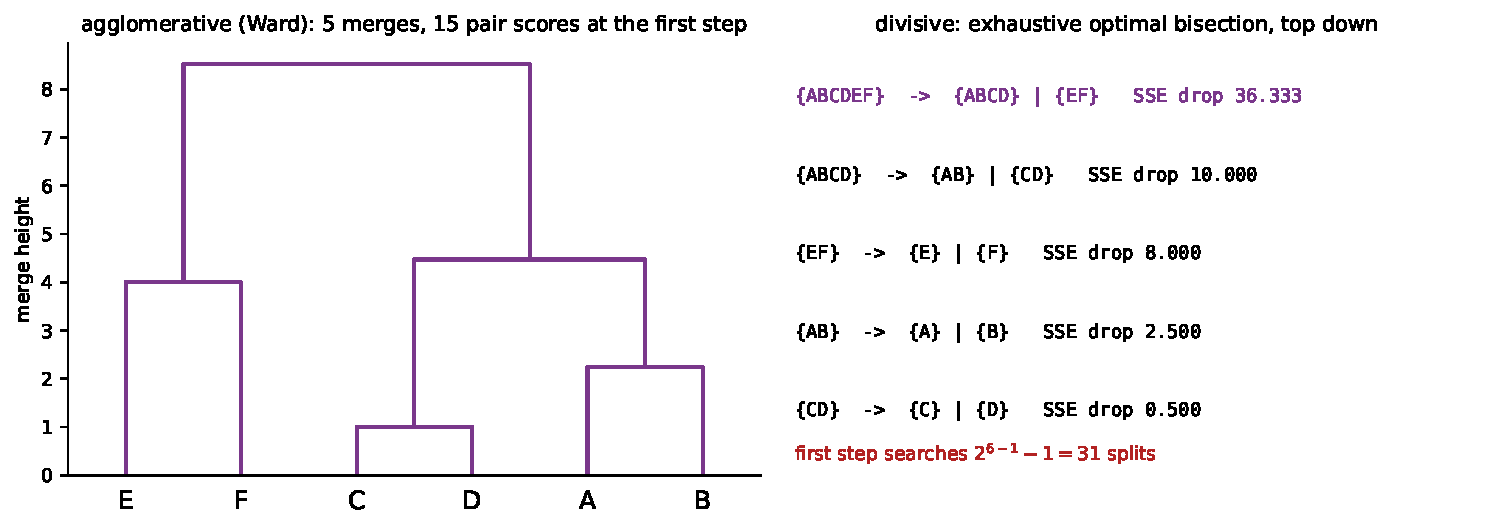
\includegraphics[width=0.68\textwidth]{updown.pdf}
  \end{center}
  \vspace{-0.2em}
  \begin{columns}[T]
    \begin{column}{0.49\textwidth}
      \begin{exampleblock}{The optimal top-down tree is the Ward tree, backwards}
        \scriptsize And the first split's SSE drop, $\mathbf{36.333}$, is
        exactly the $\Delta(\{A,B,C,D\},\{E,F\})$ we computed by hand. A happy
        accident of a small clean example --- not guaranteed in general.
      \end{exampleblock}
    \end{column}
    \begin{column}{0.49\textwidth}
\begin{outblk}
wine, 178 rows, standardised, k = 3
  Ward HAC          ARI 0.7899
  bisecting k-means ARI 0.7062
  n=8000  Ward 1.313 s
          bisecting 0.005 s  (260x)
\end{outblk}
      \begin{center}\scriptsize
        Comparable quality, two orders of magnitude faster, $O(n)$ memory.
        The exact version: Ward needs all $31{,}996{,}000$ distances first.
      \end{center}
    \end{column}
  \end{columns}
\end{frame}

\begin{frame}{So why is agglomerative the default?}
  \begin{columns}[T]
    \begin{column}{0.48\textwidth}
      \begin{block}{It is deterministic}
        Bisecting $k$-means depends on a random initialisation; run it twice
        and you may get two trees. HAC gives the same tree every time.
      \end{block}
    \end{column}
    \begin{column}{0.48\textwidth}
      \begin{block}{It gets the bottom of the tree right}
        Divisive methods make their \emph{coarsest} decisions first, on the
        least information, and a bad first split can never be repaired.
      \end{block}
    \end{column}
  \end{columns}
  \vspace{0.5em}
  \begin{exampleblock}{}
    \centering
    Care about fine structure --- which small groups are most alike? Build
    \textbf{bottom-up}. \\
    Care only about the top few levels of a large data set? Build
    \textbf{top-down}.
  \end{exampleblock}
\end{frame}

% =====================================================================
\section{Summary}
\label{sec:summary}

\begin{frame}[shrink=14]{Summary --- fourteen lines}
  \begin{enumerate}\small
    \item A hierarchical clustering is a \textbf{nested family} of partitions,
      one for every $k$, drawn as a dendrogram.
    \item Leaf order means nothing; \textbf{node heights mean everything}.
    \item HAC: start from $n$ singletons, merge the two closest clusters
      $n-1$ times. Greedy, deterministic, \textbf{irrevocable}.
    \item Its only input is the \textbf{proximity matrix} --- so it works on
      any dissimilarity, except centroid and Ward, which need Euclidean
      points.
    \item Single $= \min$, update by element-wise minimum. Complete $= \max$,
      update by element-wise maximum; the merge height is the cluster
      diameter.
    \item Same six points, different trees: $1,\ 2,\ 2.2361,\ 3.1623,\ 4$
      against $1,\ 2.2361,\ 4,\ 4.4721,\ 8.6023$.
    \item Average $=$ mean of the $n_A n_B$ cross distances; centroid
      $= \lVert c_A - c_B\rVert$; Ward $= \sqrt{2\Delta}$ for the
      within-cluster sum-of-squares increase $\Delta$.
    \item \textbf{Lance--Williams} unifies all five: one recurrence, four
      constants.
    \item Linkage encodes a belief about shape. Single: ARI $1.000$ on moons,
      ARI $0.000$ on touching blobs. Complete and Ward cut long clusters
      across the middle.
    \item \textbf{Chaining}: twelve bridge points take single linkage from
      $[60,60]$ to $[131,1]$. Complete and Ward do not move.
    \item \textbf{Centroid linkage inverts} --- $0.9675$ then $0.8683$ on
      three points --- and a non-monotone dendrogram cannot be cut.
    \item Cut by count or by height. The largest gap is a \textbf{heuristic}
      and it points at small $k$: iris says $2$, the species say $3$.
    \item Scaling and the dissimilarity matter more than the linkage: wine,
      average linkage, ARI $-0.0054$ Euclidean against $0.8224$ correlation.
    \item \textbf{Cost}: $O(n^2)$ space always. At $n = 100{,}000$ that is
      $37.3$\,GiB, and the discussion is over.
  \end{enumerate}
\end{frame}

\begin{frame}[shrink=17]{Before the next lecture}
  \begin{columns}[T]
    \begin{column}{0.49\textwidth}
      \begin{block}{Do this with a pen}
        Take any five or six objects, write the proximity matrix, and run
        \textbf{both} single and complete linkage to completion, rewriting the
        matrix after every merge. Draw both dendrograms. Then check the
        heights against \texttt{scipy.cluster.hierarchy.linkage}.

        \medskip
        This is the examinable calculation. Twenty minutes now saves you the
        marks later.
      \end{block}
    \end{column}
    \begin{column}{0.49\textwidth}
      \begin{block}{Read}
        The notes: every matrix above is written out, and the practice
        questions include three more hand runs with full solutions.
      \end{block}
      \begin{exampleblock}{Next up}
        \textbf{Partitioning and density-based clustering.} $k$-means,
        $k$-medoids, CLARA and DBSCAN --- methods that scale to the
        $200{,}000$ rows this one cannot touch, at the price of having to
        choose $k$ in advance and getting a different answer every run.
      \end{exampleblock}
    \end{column}
  \end{columns}
  \slidesources{\AMLUnitVIISources}
\end{frame}

\end{document}
